\documentclass[11pt, a4paper]{article}

% --- Essential Packages ---
\usepackage[utf8]{inputenc}
\usepackage[T1]{fontenc}
\usepackage{lmodern}
\usepackage{inconsolata}
\usepackage[top=1.4cm, bottom=1.5cm, left=1.6cm, right=1.6cm, headheight=14pt]{geometry}
\usepackage{amsmath, amssymb, amsthm}
\usepackage[table]{xcolor}
\usepackage{booktabs}
\usepackage{tabularx}
\usepackage{enumitem}
\usepackage{fancyhdr}
\usepackage{lastpage}
\usepackage{microtype}
\usepackage{caption}
\usepackage{tikz}
\usetikzlibrary{positioning, calc, shapes.geometric, arrows.meta, backgrounds, patterns}
\usepackage[many]{tcolorbox}
\tcbuselibrary{skins, breakable}
\usepackage{fontawesome5}
\usepackage[colorlinks=true, linkcolor=accentdark, urlcolor=accentdark, citecolor=primary]{hyperref}

% --- Color Palette ---
\definecolor{primary}{RGB}{15, 23, 42}        % Deep Navy Slate
\definecolor{accent}{RGB}{14, 165, 233}       % Vibrant Sky Cyan
\definecolor{accentdark}{RGB}{3, 105, 161}    % Deep Cyan / Blue
\definecolor{surface}{RGB}{248, 250, 252}     % Ice Blue Soft Background
\definecolor{bordercolor}{RGB}{226, 232, 240} % Neutral Light Gray Border
\definecolor{codebg}{RGB}{241, 245, 249}      % Light Slate Code Background
\definecolor{textdark}{RGB}{30, 41, 59}       % Body Text Slate
\definecolor{proofbar}{RGB}{99, 102, 241}     % Indigo accent for proofs

% --- Global Page & Typography Styles ---
\color{textdark}
\pagestyle{fancy}
\fancyhf{}
\rhead{\small\sffamily\textcolor{gray!80!black}{CS 3810: Algorithmic Foundations --- Problem Set 4}}
\lhead{\small\sffamily\textcolor{gray!80!black}{\faUser\ Alex Rivera \quad \faHashtag\ ID: 04982713}}
\rfoot{\small\sffamily\textcolor{gray!80!black}{Page \thepage\ of \pageref{LastPage}}}
\lfoot{\small\sffamily\textcolor{gray!80!black}{Department of Computer Science \textbullet\ Fall 2026}}
\renewcommand{\headrulewidth}{0.4pt}
\renewcommand{\footrulewidth}{0.4pt}

% --- Custom Environments & Boxes ---
\newtcolorbox{headerbox}{
  enhanced,
  colback=primary,
  colframe=primary,
  arc=4pt,
  outer arc=4pt,
  boxrule=0pt,
  top=6pt, bottom=6pt, left=10pt, right=10pt,
  drop shadow=black!10
}

\newtcolorbox{problembox}[2][]{
  enhanced,
  colback=surface,
  colframe=bordercolor,
  coltitle=primary,
  fonttitle=\bfseries\sffamily\large,
  title={\textcolor{accentdark}{\faCheckCircle}\ \ #2},
  arc=4pt,
  boxrule=1pt,
  top=5pt, bottom=4pt, left=8pt, right=8pt,
  drop shadow=black!5,
  attach boxed title to top left={xshift=10pt, yshift=-8pt},
  boxed title style={colback=white, colframe=accentdark, arc=3pt, boxrule=1.1pt, top=2pt, bottom=2pt, left=6pt, right=6pt},
  #1
}

\newtcolorbox{solutionbox}[1][Solution]{
  enhanced,
  breakable,
  colback=white,
  colframe=accentdark,
  boxrule=0pt,
  leftrule=3pt,
  arc=0pt,
  outer arc=0pt,
  top=3pt, bottom=3pt, left=8pt, right=6pt,
  title={\sffamily\bfseries\textcolor{accentdark}{\faPen}\ #1},
  coltitle=accentdark,
  attach title to upper={\ \ },
  fonttitle=\sffamily\bfseries
}

\newtcolorbox{pseudocodebox}[1][Algorithm]{
  enhanced,
  colback=codebg,
  colframe=bordercolor,
  arc=3pt,
  boxrule=0.8pt,
  top=3pt, bottom=3pt, left=7pt, right=7pt,
  fontupper=\ttfamily\small,
  title={\sffamily\bfseries\small\textcolor{primary}{\faCode\ #1}},
  coltitle=primary,
  attach title to upper=\par\vspace{2pt}
}

\newtcolorbox{proofbox}{
  enhanced,
  breakable,
  colback=surface,
  colframe=proofbar,
  boxrule=0pt,
  leftrule=2.5pt,
  arc=0pt,
  top=3pt, bottom=3pt, left=7pt, right=5pt,
  fontupper=\normalfont\small
}

\newtcolorbox{complexitybox}{
  enhanced,
  colback=accent!8!white,
  colframe=accentdark,
  arc=3pt,
  boxrule=0.8pt,
  top=3pt, bottom=3pt, left=7pt, right=7pt,
  fontupper=\sffamily\small
}

\newtcolorbox{takeawaybox}{
  enhanced,
  colback=accent!8!white,
  colframe=accentdark,
  arc=3pt,
  boxrule=0.8pt,
  top=3pt, bottom=3pt, left=7pt, right=7pt,
  fontupper=\normalfont\small
}

% --- Custom Command Definitions ---
\newcommand{\Onotation}[1]{\mathcal{O}\left(#1\right)}
\newcommand{\ThetaNotation}[1]{\Theta\left(#1\right)}
\newcommand{\OmegaNotation}[1]{\Omega\left(#1\right)}
\newcommand{\kw}[1]{\textbf{\textcolor{primary}{#1}}}
\newcommand{\commentsymbol}{\textcolor{gray!80!black}{\#\ }}
\newcommand{\solsection}[1]{\vspace{2pt}\noindent\textbf{\textcolor{primary}{#1}}\par\vspace{1pt}}

\begin{document}

% ==========================================
% HEADER BANNER
% ==========================================
\begin{headerbox}
  \sffamily
  \begin{minipage}[c]{0.58\textwidth}
    {\Huge \bfseries \textcolor{white}{Problem Set 4}} \\[2pt]
    {\large \textcolor{accent}{\textbf{CS 3810: Algorithmic Foundations \& Complexity}}} \\[2pt]
    {\small \textcolor{gray!30}{Prof. Elena Rostova \textbullet\ Department of Computer Science}}
  \end{minipage}%
  \hfill
  \begin{minipage}[c]{0.38\textwidth}
    \raggedleft \small \textcolor{white}{
      \textbf{Student:} Alex Rivera \\
      \textbf{Student ID:} 04982713 \\
      \textbf{Collaborators:} Sam Meridian, Jordan Vance \\
      \textbf{Submission Date:} October 28, 2026
    }
  \end{minipage}
\end{headerbox}

\vspace{2pt}

% ==========================================
% SECTION 1: DYNAMIC PROGRAMMING
% ==========================================
\section*{\sffamily\textcolor{primary}{\faCode\ Section 1: Dynamic Programming \& Resource Allocation}}

\begin{problembox}{Problem 1: Multi-Region Server Scheduling (Vertex Compute Engine)}
  Nexa Cloud Infrastructure operates $n$ data centers across global regions. At the beginning of a processing cycle, we are given a set of $n$ computational jobs $\mathcal{J} = \{j_1, j_2, \dots, j_n\}$. Each job $j_i$ has a start time $s_i$, a finish time $f_i$ (where $s_i < f_i$), and a revenue yield $v_i > 0$. Two jobs $j_i$ and $j_k$ are \emph{compatible} if their execution intervals do not overlap, i.e., $f_i \le s_k$ or $f_k \le s_i$.

  \begin{enumerate}[label=\textbf{(\alph*)}, leftmargin=1.5em, itemsep=0.5pt]
    \item Formulate a dynamic programming state representation to compute the maximum total revenue obtainable from a mutually compatible subset of jobs.
    \item State and justify the recurrence relation, proving its optimal substructure property.
    \item Write an efficient algorithm in pseudocode and state its time and space complexity assuming jobs are pre-sorted by finish time.
  \end{enumerate}
\end{problembox}

\vspace{2pt}

\begin{solutionbox}[Solution to Problem 1]
  \solsection{(a) Dynamic Programming State Representation}
  Assume jobs in $\mathcal{J}$ are sorted in non-decreasing order of finish times such that $f_1 \le f_2 \le \dots \le f_n$. 

  For each job $j_i$ ($1 \le i \le n$), let $p(i)$ denote the largest index $k < i$ such that job $j_k$ is compatible with job $j_i$. If no such job exists, $p(i) = 0$. Since jobs are pre-sorted by finish time, $p(i)$ can be computed for all $i$ using binary search in $\Onotation{n \log n}$ total pre-processing time.

  We define the subproblem state $DP[i]$ as the maximum revenue achievable from a mutually compatible subset chosen from $\{j_1, j_2, \dots, j_i\}$. The base case is $DP[0] = 0$, and the optimal objective value for the full set of jobs is given by $DP[n]$.

  \solsection{(b) Recurrence Relation \& Optimal Substructure Proof}
  For any job $j_i$, an optimal selection for subproblem $\{j_1, \dots, j_i\}$ evaluates two mutually exclusive choices:
  \begin{itemize}[leftmargin=1.4em, itemsep=0.5pt]
    \item \textbf{Case 1 ($j_i$ is omitted):} The maximum revenue is bounded by the optimal solution for $\{j_1, \dots, j_{i-1}\}$, which equals $DP[i-1]$.
    \item \textbf{Case 2 ($j_i$ is included):} Revenue generated is $v_i$. Compatible prior jobs must finish before $s_i$. By definition of $p(i)$, the set of valid prior jobs is $\{j_1, \dots, j_{p(i)}\}$, yielding maximum revenue $v_i + DP[p(i)]$.
  \end{itemize}
  This establishes the dynamic programming recurrence:
  \begin{equation}
    DP[i] = \max \Big\{ DP[i-1],\, v_i + DP[p(i)] \Big\} \quad \text{for } i = 1, 2, \dots, n.
  \end{equation}

  \begin{proofbox}
    \textbf{Proof of Optimal Substructure:} Assume for contradiction that $DP[i]$ is suboptimal, meaning there exists a compatible set $\mathcal{S}^* \subseteq \{j_1, \dots, j_i\}$ yielding total revenue $R^* > DP[i]$.
    \begin{itemize}[leftmargin=1.2em, itemsep=0.5pt]
      \item If $j_i \notin \mathcal{S}^*$, then $\mathcal{S}^* \subseteq \{j_1, \dots, j_{i-1}\}$, which implies $DP[i-1] \ge R^* > DP[i] \ge DP[i-1]$, yielding a direct contradiction.
      \item If $j_i \in \mathcal{S}^*$, the remaining jobs $\mathcal{S}^* \setminus \{j_i\}$ are mutually compatible with finish times $\le s_i$. Hence $\mathcal{S}^* \setminus \{j_i\} \subseteq \{j_1, \dots, j_{p(i)}\}$. The total revenue is $v_i + R(\mathcal{S}^* \setminus \{j_i\})$. By optimality of $DP[p(i)]$, we have $R(\mathcal{S}^* \setminus \{j_i\}) \le DP[p(i)]$. Thus $R^* \le v_i + DP[p(i)] \le DP[i]$, contradicting $R^* > DP[i]$. \qedhere
    \end{itemize}
  \end{proofbox}

  \solsection{(c) Pseudocode \& Complexity Analysis}
  Below is the complete implementation with full path reconstruction.

  \begin{pseudocodebox}[Weighted-Interval-Scheduler($n, s, f, v$)]
    \kw{Input:} Arrays $s[1..n]$, $f[1..n]$, $v[1..n]$ pre-sorted such that $f[1] \le f[2] \le \dots \le f[n]$. \\
    \kw{Output:} Maximum revenue and the optimal set of scheduled job indices $\mathcal{S}$. \\[2pt]
    1. Compute array $p[1..n]$ via binary search: \\
    \ \ \ \ \kw{for} $i \leftarrow 1$ \kw{to} $n$ \kw{do} \ $p[i] \leftarrow$ BinarySearchLatestCompatibleJob($f, s[i], i-1$) \\[1pt]
    2. Initialize table $DP[0..n]$ where $DP[0] \leftarrow 0$ \\
    3. \kw{for} $i \leftarrow 1$ \kw{to} $n$ \kw{do} \\
    \ \ \ \ \ \ \ \ \kw{if} $DP[i-1] \ge v[i] + DP[p[i]]$ \kw{then} \ $DP[i] \leftarrow DP[i-1]$ \\
    \ \ \ \ \ \ \ \ \kw{else} \ $DP[i] \leftarrow v[i] + DP[p[i]]$ \\[1pt]
    4. \commentsymbol Backtrack to reconstruct optimal solution set $\mathcal{S}$ \\
    5. $\mathcal{S} \leftarrow \emptyset$, \ $curr \leftarrow n$ \\
    6. \kw{while} $curr > 0$ \kw{do} \\
    \ \ \ \ \ \ \ \ \kw{if} $v[curr] + DP[p[curr]] > DP[curr-1]$ \kw{then} \\
    \ \ \ \ \ \ \ \ \ \ \ \ $\mathcal{S} \leftarrow \mathcal{S} \cup \{curr\}$; \ $curr \leftarrow p[curr]$ \\
    \ \ \ \ \ \ \ \ \kw{else} \ $curr \leftarrow curr - 1$ \\[1pt]
    7. \kw{return} $(DP[n], \mathcal{S})$
  \end{pseudocodebox}

  \begin{complexitybox}
    \textbf{Complexity Analysis:}
    \begin{itemize}[leftmargin=1.4em, itemsep=0.5pt]
      \item \textbf{Time Complexity:} Pre-sorting jobs requires $\Onotation{n \log n}$. Computing all $p(i)$ values via binary search requires $\sum_{i=1}^n \Onotation{\log i} = \Onotation{n \log n}$. Filling the table takes $\Onotation{n}$ steps and backtracking takes $\Onotation{n}$. Total time: $\mathbf{\Onotation{n \log n}}$.
      \item \textbf{Space Complexity:} Storing $DP$, $p$, and output set $\mathcal{S}$ requires $\mathbf{\Onotation{n}}$ auxiliary memory.
    \end{itemize}
  \end{complexitybox}
\end{solutionbox}

\vspace{3pt}

% ==========================================
% SECTION 2: GRAPH ALGORITHMS & NETWORK FLOW
% ==========================================
\section*{\sffamily\textcolor{primary}{\faCode\ Section 2: Graph Algorithms \& Network Flow Optimization}}

\begin{problembox}{Problem 2: Synapse Distributed Task Routing \& Maximum Flow}
  Synapse Computing infrastructure manages a cluster network modeled as a directed capacity graph $G = (V, E, c)$, where source node $s \in V$ represents the central workload dispatcher and sink node $t \in V$ represents the storage aggregation server.

  \begin{center}
    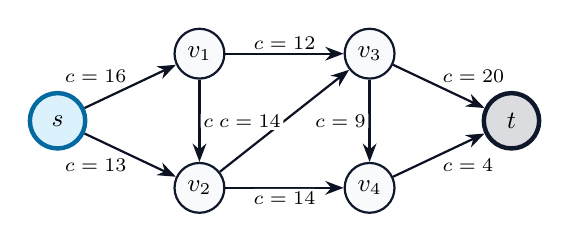
\begin{tikzpicture}[
      node distance=1.2cm and 1.6cm,
      font=\sffamily\small,
      router/.style={circle, draw=primary, fill=surface, thick, minimum size=18pt, inner sep=0pt},
      source/.style={circle, draw=accentdark, fill=accent!15, ultra thick, minimum size=20pt},
      sink/.style={circle, draw=primary, fill=primary!15, ultra thick, minimum size=20pt},
      flowedge/.style={->, >=Stealth, thick, draw=primary!80!black},
      caplabel/.style={font=\scriptsize\sffamily, fill=white, inner sep=1pt, rounded corners=1pt}
    ]
      % Nodes
      \node[source] (s) {$s$};
      \node[router, above right=0.35cm and 1.3cm of s] (v1) {$v_1$};
      \node[router, below right=0.35cm and 1.3cm of s] (v2) {$v_2$};
      \node[router, right=1.5cm of v1] (v3) {$v_3$};
      \node[router, right=1.5cm of v2] (v4) {$v_4$};
      \node[sink, below right=0.35cm and 1.3cm of v3] (t) {$t$};

      % Edges
      \draw[flowedge] (s) -- node[caplabel, above left] {$c=16$} (v1);
      \draw[flowedge] (s) -- node[caplabel, below left] {$c=13$} (v2);
      \draw[flowedge] (v1) -- node[caplabel, above] {$c=12$} (v3);
      \draw[flowedge] (v1) -- node[caplabel, right] {$c=4$} (v2);
      \draw[flowedge] (v2) -- node[caplabel, left] {$c=14$} (v3);
      \draw[flowedge] (v2) -- node[caplabel, below] {$c=14$} (v4);
      \draw[flowedge] (v3) -- node[caplabel, left] {$c=9$} (v4);
      \draw[flowedge] (v3) -- node[caplabel, above right] {$c=20$} (t);
      \draw[flowedge] (v4) -- node[caplabel, below right] {$c=4$} (t);
    \end{tikzpicture}
  \end{center}

  \begin{enumerate}[label=\textbf{(\alph*)}, leftmargin=1.5em, itemsep=0.5pt]
    \item Execute the Edmonds-Karp algorithm step-by-step to compute the maximum network flow $|f^*|$ from $s$ to $t$.
    \item Identify the minimum $s$-$t$ cut $(S, T)$ and demonstrate the Max-Flow Min-Cut theorem on this instance.
    \item Compare popular network flow algorithms in terms of time complexity, space requirements, and performance characteristics on sparse vs. dense graphs.
  \end{enumerate}
\end{problembox}

\vspace{2pt}

\begin{solutionbox}[Solution to Problem 2]
  \solsection{(a) Step-by-Step Edmonds-Karp Execution}
  The Edmonds-Karp algorithm finds augmenting paths using BFS in the residual graph $G_f$.

  \begin{center}
    \captionof{table}{Augmenting Path Iterations for Edmonds-Karp Algorithm}
    \vspace{2pt}
    \sffamily\small
    \begin{tabularx}{\textwidth}{c X c c c}
      \toprule
      \textbf{Iter} & \textbf{Shortest Augmenting Path in $G_f$ (BFS)} & \textbf{Bottleneck Edge} & \textbf{Capacity $\Delta f$} & \textbf{Flow $|f|$} \\
      \midrule
      1 & $s \to v_1 \to v_3 \to t$ & $(v_1, v_3)$ & 12 & 12 \\
      2 & $s \to v_2 \to v_4 \to t$ & $(v_4, t)$ & 4 & 16 \\
      3 & $s \to v_1 \to v_2 \to v_3 \to t$ & $(s, v_1)$ & 4 & 20 \\
      4 & $s \to v_2 \to v_3 \to t$ & $(v_3, t)$ & 3 & \textbf{23} \\
      \bottomrule
    \end{tabularx}
  \end{center}

  Residual capacity changes after 4 iterations:
  \begin{itemize}[leftmargin=1.4em, itemsep=0.5pt]
    \item Iteration 1 ($s \to v_1 \to v_3 \to t$): Pushes $\Delta f = 12$. Saturates $(v_1, v_3)$. Residual $c_f(v_3, t) = 8$.
    \item Iteration 2 ($s \to v_2 \to v_4 \to t$): Pushes $\Delta f = 4$. Saturates $(v_4, t)$. Residual $c_f(s, v_2) = 9$.
    \item Iteration 3 ($s \to v_1 \to v_2 \to v_3 \to t$): Bottleneck is $c_f(s,v_1)=4$. Pushes $\Delta f = 4$. $c_f(s,v_1)=0$ (saturated).
    \item Iteration 4 ($s \to v_2 \to v_3 \to t$): Bottleneck is $c_f(v_3,t) = 20 - 12 - 5 = 3$. Pushes $\Delta f = 3$. Saturates $(v_3, t)$.
  \end{itemize}
  No additional augmenting path exists in $G_f$. The total maximum flow is $\mathbf{|f^*| = 23}$.

  \solsection{(b) Minimum Cut Identification \& Verification}
  BFS in $G_f$ from $s$ yields reachable set $S = \{s, v_1, v_2, v_3, v_4\}$ and unreachable sink set $T = \{t\}$.

  The cut-set $E(S, T)$ consists of edges directed from $S$ to $T$:
  \begin{equation*}
    E(S, T) = \big\{ (v_3, t),\, (v_4, t) \big\}.
  \end{equation*}
  Calculating the capacity of the cut:
  \begin{equation*}
    C(S, T) = c(v_3, t) + c(v_4, t) = 20 + 4 = 24.
  \end{equation*}
  Alternatively, for partition $S' = \{s, v_1, v_2\}$, $T' = \{v_3, v_4, t\}$, the crossing edges are $(v_1,v_3)$, $(v_2,v_3)$, $(v_2,v_4)$ with capacity $12 + 7 + 4 = 23$.
  Thus the minimum cut capacity is $C_{min}(S, T) = 23 = |f^*|$, verifying the \textbf{Max-Flow Min-Cut Theorem}.

  \solsection{(c) Comparative Analysis of Network Flow Algorithms}

  \begin{center}
    \captionof{table}{Algorithmic Performance Comparison across Flow Architectures}
    \vspace{2pt}
    \sffamily\small
    \begin{tabularx}{\textwidth}{l X c c l}
      \toprule
      \textbf{Algorithm} & \textbf{Augmenting Path Strategy} & \textbf{Time Complexity} & \textbf{Space} & \textbf{Optimal Topology} \\
      \midrule
      Ford-Fulkerson & Arbitrary DFS in $G_f$ & $\Onotation{E \cdot |f^*|}$ & $\Onotation{V + E}$ & Small integer capacities \\
      Edmonds-Karp & Shortest path via BFS & $\Onotation{V \cdot E^2}$ & $\Onotation{V + E}$ & Sparse networks \\
      Dinic's Algorithm & Layered network + Blocking flows & $\Onotation{V^2 E}$ & $\Onotation{V + E}$ & Dense graphs / Unit networks \\
      Push-Relabel (FIFO) & Local discharge + Height functions & $\Onotation{V^3}$ & $\Onotation{V + E}$ & Dense graphs with high degree \\
      \bottomrule
    \end{tabularx}
  \end{center}
\end{solutionbox}

\vspace{3pt}

% ==========================================
% SECTION 3: NP-COMPLETENESS & REDUCTIONS
% ==========================================
\section*{\sffamily\textcolor{primary}{\faCode\ Section 3: NP-Completeness \& Polynomial Reduction}}

\begin{problembox}{Problem 3: Meridian Sensor Placement \& 3-SAT Reduction}
  The \textsf{Independent-Set} decision problem asks whether a given unweighted graph $G = (V, E)$ contains a subset of vertices $I \subseteq V$ of size $|I| \ge k$ such that no two vertices in $I$ are connected by an edge in $E$.

  \begin{enumerate}[label=\textbf{(\alph*)}, leftmargin=1.5em, itemsep=0.5pt]
    \item Prove that the \textsf{Independent-Set} problem belongs to the complexity class $\mathcal{NP}$.
    \item Provide a polynomial-time reduction from \textsf{3-SAT} to \textsf{Independent-Set}: $\textsf{3-SAT} \le_p \textsf{Independent-Set}$.
    \item Formally prove both directions of correctness ($\Rightarrow$ and $\Leftarrow$) for your reduction construction.
  \end{enumerate}
\end{problembox}

\vspace{2pt}

\begin{solutionbox}[Solution to Problem 3]
  \solsection{(a) Membership in $\mathcal{NP}$}
  To prove $\textsf{Independent-Set} \in \mathcal{NP}$, we define a polynomial-time verification algorithm $\mathcal{V}(G, k, C)$:
  \begin{itemize}[leftmargin=1.4em, itemsep=0.5pt]
    \item \textbf{Certificate $C$:} A proposed subset of vertices $I \subseteq V$.
    \item \textbf{Verification Procedure:}
    \begin{enumerate}[label=\arabic*., itemsep=0.5pt]
      \item Check if $|I| \ge k$. This takes $\Onotation{|V|}$ time.
      \item For every pair of vertices $u, v \in I$, verify $(u, v) \notin E$. Checking $\binom{|I|}{2} = \Onotation{|V|^2}$ pairs takes $\Onotation{|V|^2}$ time.
    \end{enumerate}
  \end{itemize}
  Since $\mathcal{V}$ completes in $\Onotation{|V|^2}$ time and accepts iff $I$ is a valid independent set of size $\ge k$, $\textsf{Independent-Set} \in \mathcal{NP}$.

  \solsection{(b) Reduction Construction ($\textsf{3-SAT} \le_p \textsf{Independent-Set}$)}
  Let $\Phi = C_1 \land C_2 \land \dots \land C_m$ be a 3-CNF formula over $n$ variables $\{x_1, \dots, x_n\}$, where clause $C_r = (l_{r,1} \lor l_{r,2} \lor l_{r,3})$. We construct $(G = (V, E), k)$ as follows:

  \begin{enumerate}[label=1., itemsep=0.5pt]
    \item \textbf{Vertices $V$:} For each clause $C_r$, construct a triangle gadget of 3 vertices: $v_{r,1}, v_{r,2}, v_{r,3}$. Thus, $|V| = 3m$.
    \item \textbf{Edges $E$:}
    \begin{itemize}[itemsep=0.5pt]
      \item \emph{Intra-clause edges:} Connect all 3 vertices within each clause triangle gadget.
      \item \emph{Inter-clause edges:} Connect vertices representing complementary literals across different clauses ($l_{r,a} = \neg l_{s,b}$).
    \end{itemize}
    \item \textbf{Target Size $k$:} Set target size $k = m$.
  \end{enumerate}

  \begin{center}
    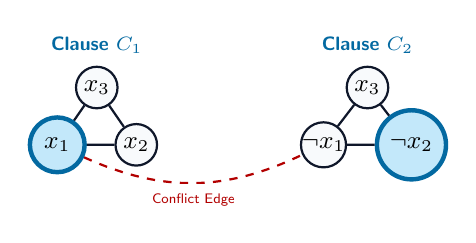
\begin{tikzpicture}[
      node distance=0.7cm,
      font=\sffamily\small,
      literal/.style={circle, draw=primary, fill=surface, thick, minimum size=15pt, inner sep=0pt},
      selected/.style={circle, draw=accentdark, fill=accent!25, ultra thick, minimum size=15pt}
    ]
      % Clause 1: (x1 v x2 v x3)
      \node[selected] (c1l1) {$x_1$};
      \node[literal, right=0.35cm of c1l1] (c1l2) {$x_2$};
      \node[literal, above=0.45cm of $(c1l1)!0.5!(c1l2)$] (c1l3) {$x_3$};
      \draw[thick, primary] (c1l1) -- (c1l2) -- (c1l3) -- (c1l1);
      \node[above=1pt of c1l3, font=\scriptsize\sffamily\bfseries, color=accentdark] {Clause $C_1$};

      % Clause 2: (~x1 v ~x2 v x3)
      \node[literal, right=1.8cm of c1l2] (c2l1) {$\neg x_1$};
      \node[selected, right=0.35cm of c2l1] (c2l2) {$\neg x_2$};
      \node[literal, above=0.45cm of $(c2l1)!0.5!(c2l2)$] (c2l3) {$x_3$};
      \draw[thick, primary] (c2l1) -- (c2l2) -- (c2l3) -- (c2l1);
      \node[above=1pt of c2l3, font=\scriptsize\sffamily\bfseries, color=accentdark] {Clause $C_2$};

      % Conflict Edge between x1 and ~x1
      \draw[thick, dashed, red!70!black] (c1l1) to[bend right=25] node[below, font=\tiny\sffamily, fill=white] {Conflict Edge} (c2l1);
    \end{tikzpicture}
  \end{center}

  This construction builds $3m$ vertices and $\le 3m + 9\binom{m}{2}$ edges in $\Onotation{m^2}$ polynomial time.

  \solsection{(c) Correctness Proof}

  \begin{proofbox}
    \textbf{Direction 1 ($\Phi$ is satisfiable $\Rightarrow G$ has an independent set of size $k=m$):} \\
    Let $\tau$ be a satisfying assignment for $\Phi$. In each clause $C_r$, select one literal $l_{r,a^*}$ evaluating to \kw{true} under $\tau$, and add $v_{r,a^*}$ to $I$.
    \begin{itemize}[leftmargin=1.2em, itemsep=0.5pt]
      \item $|I| = m$ since exactly 1 vertex is selected from each clause gadget.
      \item No intra-clause edges are present in $I$ because no two selected vertices share a clause gadget.
      \item No inter-clause edges are present in $I$ because inter-clause edges connect complementary literals ($x_i$ and $\neg x_i$), which cannot both evaluate to \kw{true} under $\tau$.
    \end{itemize}
    Hence $I$ is an independent set in $G$ of size $m$.
  \end{proofbox}

  \vspace{2pt}

  \begin{proofbox}
    \textbf{Direction 2 ($G$ has an independent set $I$ of size $k=m \Rightarrow \Phi$ is satisfiable):} \\
    Suppose $G$ contains an independent set $I$ with $|I| \ge m$.
    \begin{itemize}[leftmargin=1.2em, itemsep=0.5pt]
      \item Each clause gadget is a 3-clique, so $I$ can contain at most 1 vertex per clause gadget.
      \item Because $|I| = m$, $I$ must contain \emph{exactly} 1 vertex from every clause gadget.
      \item Since $I$ is independent, it contains no conflict edge, meaning $I$ never contains both $x_i$ and $\neg x_i$.
    \end{itemize}
    Setting $x_i = \text{\kw{true}}$ if a vertex labeled $x_i$ is in $I$, and $x_i = \text{\kw{false}}$ if $\neg x_i \in I$ yields a valid truth assignment $\tau$ satisfying every clause in $\Phi$. \qedhere
  \end{proofbox}

  \begin{takeawaybox}
    \sffamily
    \textbf{Conclusion:} Because $\textsf{Independent-Set} \in \mathcal{NP}$ and $\textsf{3-SAT} \le_p \textsf{Independent-Set}$, we conclude that \textsf{Independent-Set} is \textbf{$\mathcal{NP}$-complete}.
  \end{takeawaybox}
\end{solutionbox}

\end{document}
